\begin{comment}
* Declare some sort or terminology when referring to each simulation run inside Monte Carlo:
    - One Monte Carlo (MC) run corresponds to multiple gnss-r formation flying simulations, or simply multiple simulation runs. 
    - Simulator is used to refer to the entire thing, which is the same as saying one MC run. 
\end{comment}


\section{Simulation Architecture}

\begin{figure}[H]
    \centering
    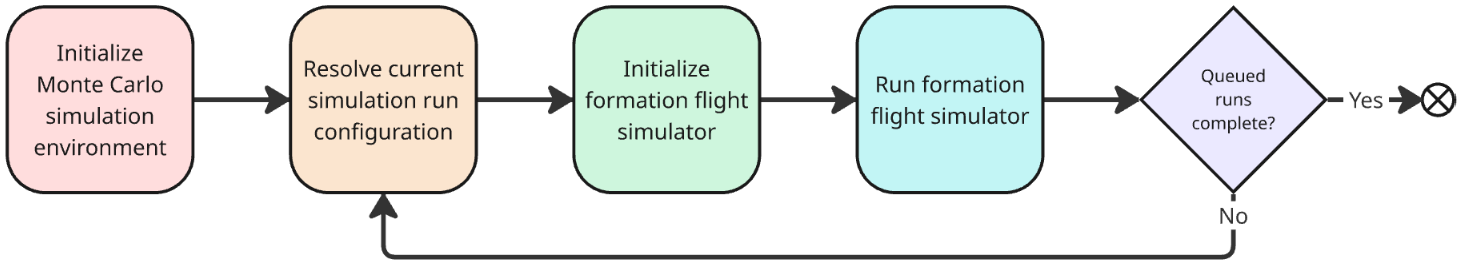
\includegraphics[width=0.8\textwidth]{Figures/04Method/Abstracted formation flight simulator.png}
    \caption{Simplified GNSS-R formation flight simulator flow diagram}.
    \label{fig:simple_formfly_flow} 
\end{figure}

The high-level execution flow of the GNSS-R Formation Flight Simulator is shown in Figure \ref{fig:simple_formfly_flow}. The simulator is organized into five main program blocks: initialization of the \gls{mc} simulation environment, resolution of the current simulation run configuration, initialization of the formation flight simulator, execution of the formation flight simulator, and evaluation of whether additional \gls{mc} runs remain. These blocks can be divided into two main parts, separated by the vertical dashed line in the detailed flowchart in Figure \ref{fig:formfly_flow}. The left part acts as a simulation run orchestrator, where the \gls{mc} environment is configured, and run-specific configuration files are prepared. The right part represents the iterative execution of individual simulation runs, where each run is initialized, executed, and written to file before the next queued run is started. As in the Comparative Propagation Simulator architecture presented in Section \ref{sec:propagator_architecture}, the detailed flowchart is divided into vertically stacked layers representing input files, internal object instances, program blocks, transferred output objects, and generated output files. However, unlike the Comparative Propagation Simulator, the GNSS-R Formation Flight Simulator does not include a separate Skyfield propagation module, but is built entirely around Basilisk numerical simulation.

\begin{figure}[H]
    \centering
    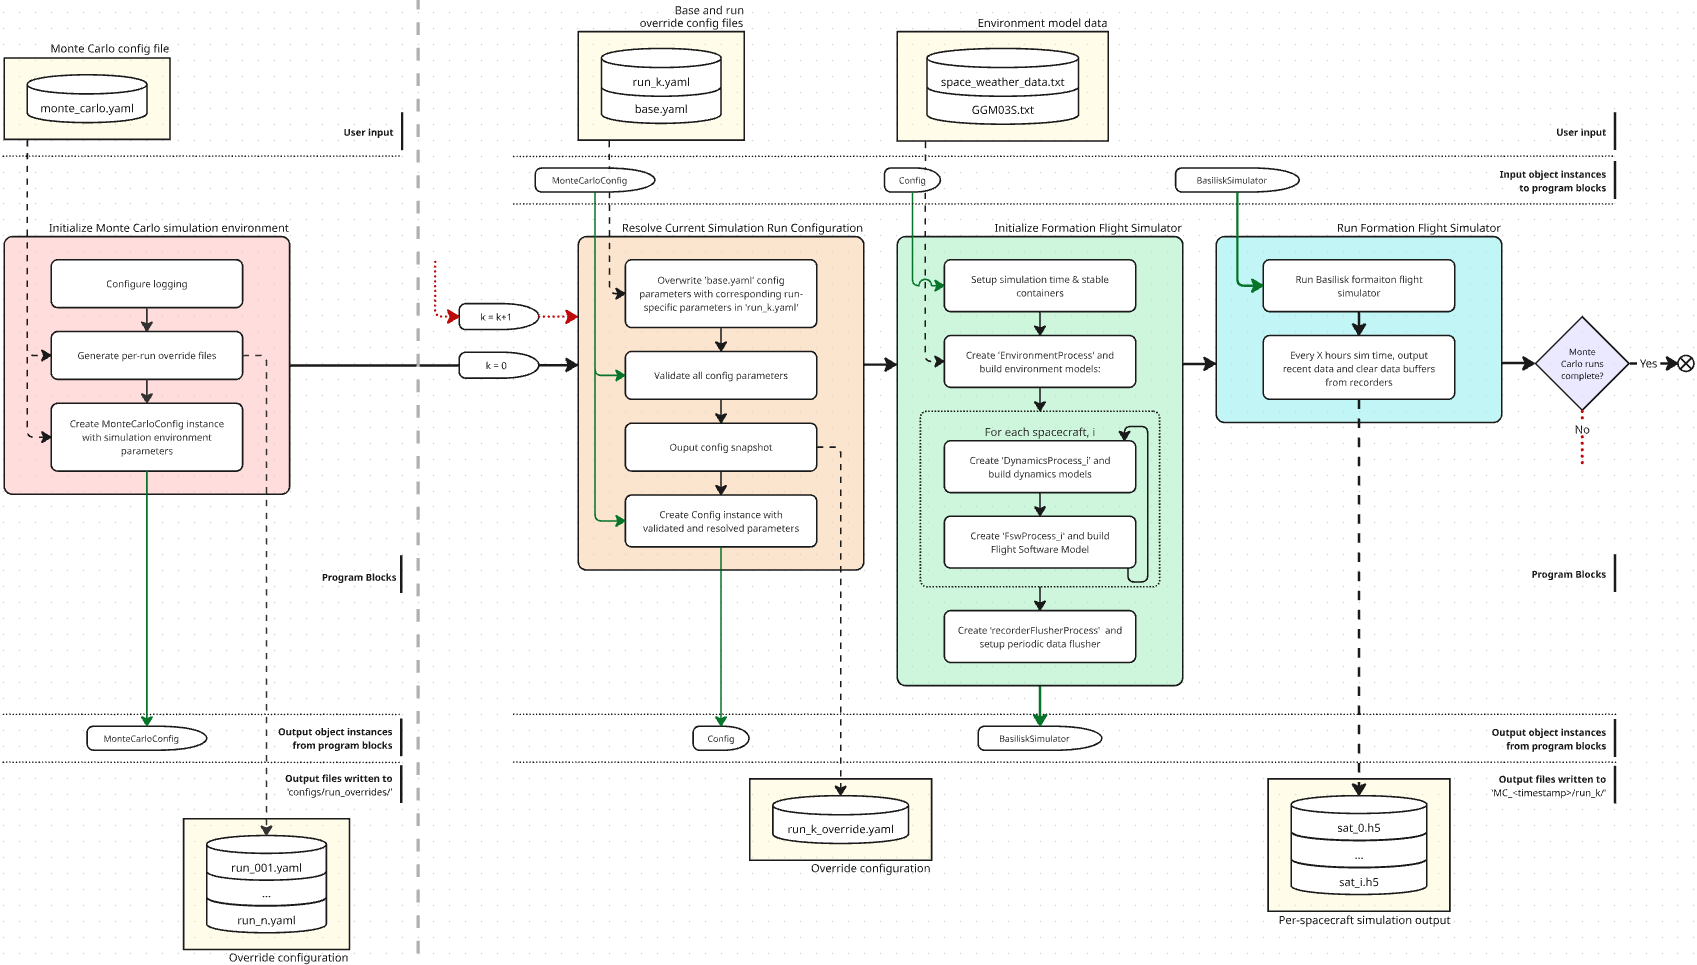
\includegraphics[width=1.0\textwidth]{Figures/04Method/Formation Flight Simulator.png}
    \caption{Detailed GNSS-R formation flight simulator flow diagram}.
    \label{fig:formfly_flow} 
\end{figure}

\subsection{Initialization of the Monte Carlo Environment}
The first program block initializes the \gls{mc} simulation environment from the user-defined configuration file \texttt{monte\_carlo.yaml}, and is considered the simulation run orchestrator. In this thesis, \gls{mc} execution is assumed to be enabled for all simulation cases, such that the simulator is structured around a queue of formation-flight simulation runs rather than a single isolated run. The \gls{mc} configuration defines the number of queued runs and the run-specific parameter variations used to generate override configuration files. If $n$ simulation runs are queued, $n-1$ override files are generated. Finally, the validated \gls{mc} settings are collected into a global \gls{mc} configuration instance, which is passed to the iterative part of the simulator and determines how the queued formation-flight simulations are executed.


\subsection{Current Run Configuration Resolution}
The next program block resolves the configuration for the current simulation run. This step is similar to the configuration initialization used in the Comparative Propagation Simulator, described in Section \ref{sec:propagator_init}, but is extended to support iterative \gls{mc} execution. For the first simulation run, the configuration is defined directly by the default scenario in \texttt{base.yaml}. For all subsequent runs, the corresponding override file \texttt{run\_k.yaml} is loaded and used to replace selected parameters in \texttt{base.yaml}, where $k$ denotes the current simulation run index. This allows each queued run to modify a limited set of scenario parameters while preserving the remaining default configuration. Once the current run configuration has been resolved, all parameters are validated and written to a timestamped configuration snapshot. As in the Comparative Propagation Simulator, this snapshot provides traceability by allowing each generated output data set to be linked to the exact parameter values used to produce it. Finally, the validated parameters are collected into a run-specific \texttt{Config} instance, which is passed to the formation flight simulator initialization block.


\subsection{}



\begin{comment}
This section should explain the high-level flow of the gnss-r formation flight simulator. It should contain the following:
* 1st paragraph:
    - Just like in the corresponding section for the other simulator, start by explaining the main modules aka. program blocks of the simulator, which is clearly shown in Figure \ref{fig:simple_formfly_flow} (the same program blocks is shown in \ref{fig:formfly_flow, but it is harder to make out})
        1. Setting up the Monte Carlo simulation environment
        2. Resolve current simulation run configuration
        3. Initialize formation flight simulator
        4. Run formation flight simulator
        5. Repeat from 2 if there are more simulations queued in the Monte Carlo run. 
    - The main modules can therefore be divided into two sections, which is divided by the vertical dotted line in the flowchart \ref{fig:formfly_flow}: the simulation run orchestrator on the left, and the iterative simulation runs on the right. 
    - The flowchart is also divided into different vertically stacked layers. Just like in Section \ref{sec:propagator_architectur}, the top and bottom layers represent the input and output files, the middle layer shows the program blocks, and the adjacent layers show how object instances are passed between them. Though, it is important to note that the left and right sections output files to different directories. 
    - Point out that, unlike the other simulator, the gnss-r formation flight simulator does not include its own skyfield module, but is entirely built upon the Basilisk framework. 

* 2nd paragraph (Initialization of the Monte Carlo environment)
    - The Monte Carlo (MC) initialization program block is responsible for defining the global Monte Carlo configuration from user input (\texttt{monte_carlo.yaml}).
    - After the \gls{mc} configuration file is loaded, it is used to generate n override configuration files, where n denotes the number of queued simulation runs-1.
    - Each override configuration file contain any number of parameters that override the default scenario, which enables the changing different scenario parameters between queued simulation runs.
    - Finally, the loaded monte carlo configuration file is used to create a global MonteCarloCondig.

* 3rd paragraph (Current run configuration resolution)
    - Explains how the "Resolve current simulation run configuration" program block works:
    - This is very similar to the initialization of the simulation environment program block described in Section \ref{sec:propagator_init}. The only substantial difference is that the iterative runs require resolving a combination of parameters from default.yaml, and run_k.yaml
    - This is the first step of this program block. For the very first simulation run, only the configuration parameters from \texttt{default.yaml} are used, but in every other following runs (k != 0), the parameters in run_k.yaml override the corresponding parameters in base.yaml. 
    - Then all resolved config parameters are validated, before a snapshot of the simulation configuration is exported. As mentioned before, this is important for traceability because it allows checking what parameters were used to generate an output data set at a later time. 
    - Finally, the validated parameters are  collected into a Config instance 


* 4th paragraph
    - Explains how the current run Basilisk GNSS-R formation flight simulator is initialized and run.
    - state that this high-level flow is very similar to "Basilisk Propagator Flow" presented in Section \ref{sec:basilisk_propagator_flow}


For later paragraphs: (avoid for now)
    Should be compared to the propagator simulator because this is an expansion/re-structured variant
    * Like in the Comparative propagation simulator "simulation architecture" section, this section should start by explaining the main program blocks by referencing the flow diagram \ref{fig:formfly_flow}. 
    * Task/process structure and resulting execution order
    * State that the old super-process has been split into environment and dynamics processes
    * Explain what each process is responsible for 
    * Conclude by saying that although this flowchart nicely presents the high-level simulator flow, it hides the inner complexity of the GNSS-R GNC modules. This will be explored in further detail in the coming sections. 

\end{comment}




\section{Electronic Power System}
\begin{comment}
Consumers and generators of electricity. How these effect battery, and how battery thresholds are defined. 
\end{comment}


\section{Flight Software}
\begin{comment}
* Overall structure, how is it all connected and run during execution
* Guidance pointing logic w. all states and mode transitions
* MRP feedback pointing controller 
* Formation control 
\end{comment}

\subsection{Software Architecture}

\subsection{Pointing Guidance Logic}

\subsection{MRP Feedback Pointing Controller}

\subsection{Formation Controller}

\section{Simulator inputs}

\begin{figure}[htbp]
    \small
    \dirtree{%
    .1 GNSS-R Formation Flight Simulator.
    .2 EnvironmentProcess.
    .3 EnvironmentTask.
    .4 spiceObj [20].
    .4 eclipseObj [20].
    .4 groundStation(s) [20].
    .4 atmObj [20].
    .3 MsisInputUpdaterTask.
    .4 msisInputUpdater [20].
    .2 DynamicsProcess\_\textless sat\_idx\textgreater.
    .3 DynamicsTask\_\textless sat\_idx\textgreater.
    .4 scObj.
    .4 dragEffector [20].
    .4 srpEffector [20] .
    .4 solarPanel(s) [20].
    .4 rwEffector [20].
    .4 thrusterEffector [20].
    .4 fuelTankEffector [20].
    .4 battery [20].
    .4 obcPowerSink [20].
    .4 rwPower(s) [20].
    .4 thrusterStateRecorder [10].
    .4 fuelTankStateRecorder [10].
    .4 rwStateRecorder(s) [10].
    .4 rwStateRecorder(s) [10].
    .4 batteryStateRecorder [10].
    .4 obcPowerSinkRecorder [10].
    .4 solarPanelPowerRecorders(s) [10].
    .2 FswProcess\_\textless sat\_idx\textgreater.
    .3 FswTask\_\textless sat\_idx\textgreater.
    .4 scheduler [20].
    .4 navTransRecorder [10].
    .4 navAttRecorder [10].
    .4 attRefRecorder [10].
    .4 attErrRecorder [10].
    .4 cmdTorqueRecorder [10].
    .4 rwMotorTorqueRecorder [10].
    .2 RecorderFlusherProcess.
    .3 RecorderFlusherTask [20].
    .4 recorderFlusher [20].
    }
    \caption{Hierarchical process-task-model structure of the GNSS-R formation flight Basilisk simulator. The number in square brackets denote the model priority, where higher priority models are updated first. Same-priority tasks are orderly updated from the top-down within a task. ''\textit{<sat\_idx>}'' represent per-spacecraft processes and tasks.}
    \label{fig:basilisk_simulator_hierarchy}
\end{figure}
